
\chapter{Effizientes Sortieren und Suchen}
in $\bigO{}(N)$ (Sortieren) bzw. $\bigO{}(1)$ (Suchen) \\
\begin{itemize}[label={}]
    \item \textbf{Beweis} wenn man nur die Operation \verb|key1 < key2| (Ordnung) zur Verfügung hat, ist Sortieren nicht besser als $\Omega (NlogN)$ möglich
    \item \textbf{Beispiel} Array der Länge 3: kann in $ 6 = 3!$ verschiedenen Sortierungen vorliegen: ABC, ACB, BAC, BCA, CAB, CBA \\
    Ratespiel: mit möglichst wenigen Fragen herausfinden, welche Permutation vorliegt $\Rightarrow$ Suchbaum, Fragebaum \\
    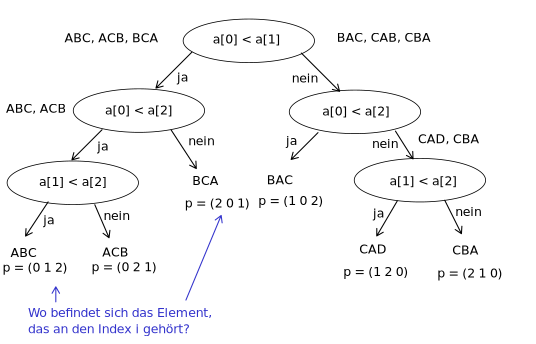
\includegraphics[width=16cm,height=6cm,keepaspectratio]{./Pictures/Fragebaum.png}
\end{itemize}
wenn man p kennt, kann man in $\bigO{}(N)$ sortieren
\begin{minted}{python}
def index_sort(a, p):
    v = [None] * len(a)
    for k in range(len(a)): v[k] = a[p[k]] #O(N)
    return v
\end{minted}
\vspace*{0.5cm}
Wie groß ist der Fragebaum mindestens, wenn wir die Frage so geschickt wie möglich stellen?
\begin{itemize}[label={}]
    \item Um N! Permutationen zu repräsentieren, brauchen wir N! Blätter
    \item Um N! Blätter zu haben, muss der Baum die Tiefe $\Omega (log N!)$ haben
    \item Vereinfachen mit Hilfe der Stirlingschen Formel für große N:
    \[ N! \approx \sqrt{2 \pi N} * \left( \frac{N}{e}\right) ^N\]
    \[ log\hspace*{1mm}N! \approx log\hspace*{1mm} \sqrt{2\pi N} + log\hspace*{1mm} N^N - log\hspace*{1mm} e^N \geq log\hspace*{1mm} \sqrt{2\pi N} + log\hspace*{1mm} N^N\]
    \[ \Omega(log\hspace*{1mm}N!) = \Omega(log\sqrt{2\pi N}) + \Omega(log\hspace*{1mm}N^N) = \boxed{\Omega(N \hspace*{1mm}log\hspace*{1mm}N)}\]
    \item $\Rightarrow$ Sortieren allein mit paarweisen Vergleichen \verb|"key1 < key2"| braucht immer mindestens $\Omega(N \hspace*{1mm} log \hspace*{1mm}N)$ Zeit
    \item $\Rightarrow$ Merge Sort, Quick Sort, Heap Sort sind nicht zu verbessern, ohne zusätzliche Anforderungen in die Schlüssel
\end{itemize}

\section{Sortieren in linearer Zeit $\bigO{}$(N)}
\begin{itemize}
    \item ist einfach, wenn die Schlüssel ganze Zahlen im Bereich $[0, \cdots, M-1]$ \\
    so dass $M \in \bigO{}(N)$ $\Rightarrow$ benutze Array($\infty$) von Arrays $\rightarrow$ ein Array pro Schlüssel (genauer: Queue)
\end{itemize}
\begin{minted}{python}
def integer_sort(a, M):
    bucket = [ [] for k in range(M)] #M leere Queues ([])
    #M = Anzahl der erlaubten Schluessel
    #verteile Raten auf Buckets
    for k in range(len(a)):
        bucket[a[k]._key].append(a[k])  #a[k]._key Element von [0, M-1]

    # sortiertes Array aus den Queues zusammensetzen
    start = 0
    for k in range(M):
        end = start + len(bucket[k])
        [a[start:end] = bucket[k]   #alle Elemente mit Schluessel k in a sortiert einfuegen
        start = end
\end{minted}
Komplexität
\begin{itemize}
    \item line 1-3: $\bigO{}(M)$
    \item line 4-6: $\bigO{}(N)$
    \item line 10-13: $\bigO{}(N) \begin{cases} \text{line 11}: \bigO{}(k) \\ \text{line 12}: \bigO{}(N_k) \\ \text{line 13}: \bigO{}(1) \end{cases}$
\end{itemize}
Schleife über Buckets hat Komplexität: \[\sum_{\Psi = 0}^{M-1} \bigO{}(N_k) = \bigO{}\underbrace{\left(\sum_{k = 0}^{M-1}N_k\right)}_{=N} = \bigO{}(N)\]

$\Rightarrow$ der gesamte Algorithmus ist $\bigO{}(N)$, falls $M \in \bigO{}(N)$ \\

\subsubsection*{Wie kann man das auf beliebige Schlüssel verallgemeinern?}
\begin{itemize}
\item Quantisierung: \verb|quantize(key, M)| $\Rightarrow$ \verb|[0, M-1]| $\widehat{=} q_{\text{key}}$ \\
\hspace*{0.1cm} Ordnungserhaltend: falls \verb|key1| $<$ \verb|key2| $\Rightarrow$ $q_{\text{key1}} \leq q_{\text{key2}}$ \\
wenn eine solche Funktion für keys definiert ist $\Rightarrow$ bucket sort $\in \bigO{}(N)$
\end{itemize}

\section{Bucket Sort}

\begin{minted}{python}
def bucket_sort(a, quantize, d):
    N = len(a)
    M = int(N / float(d)) #Python3 N//d
    # M = Anzahl der Buckets, d = mittlere Zahl von Elementen in jedem Bucket

    bucket = [[] for k in range(M)]
    #Daten auf buckets verteilen
    for k in range(N):
        index = quantize(a[k]._key, M)
        bucket[index].append(a[k])
    #Daten sortiert einfuegen
    start = 0
    for k in range(M):
        insertion_sort(bucket[k])   #sortiere Schluessel mit gleicher Quantisierung
        end = start + len(bucket[k])
        a[start:end] = bucket[k]
        start = end
\end{minted}
Komplexität:
\begin{itemize}
    \item line 2: $\bigO{}(1)$
    \item line 3: $\bigO{}(1)$
    \item line 6: $\bigO{}(M)$
    \item line 8-10 : $\bigO{}(N) \begin{cases}\text{line 8: } \bigO{}(N) & \\ \text{line 9: } \bigO{}(1) & ! \\ \text{line 10: }  \bigO{}(1) & \text{amortisiert}\end{cases}$
    \item line 12: $\bigO{}(1)$
    \item line 13 - 17: $\sum_{k=0}^{M-1} \bigO{}(N_k^2) \begin{cases} \text{line 13: } & \bigO{}(M) \\ \text{line 14: } & \bigO{}(N_k^2) \\  \text{line 15: } & \bigO{}(1)  \\\text{line 16: } & \bigO{}(N_k) \\  \text{line 17: } & \bigO{}(1) \\ \end{cases}$
\end{itemize}
zum Vergleich: integer\_sort:
\[ \sum_{k=0}^{M-1} \bigO{}(N_k) = \bigO{}\left( \sum_{k=0}^{M-1} N_k\right) = \bigO{}(N)\]

jetzt:
\[ \sum_{k=0}^{M-1} \bigO{}(N_k^2) = \sum_{k=0}^{M-1} \bigO{}(1) = \bigO{}(M) \hspace*{0.5cm} \underline{\text{falls }} N_k \in \bigO{}(1) \text{, d.h. unabh. von N und M} \]

\textbf{Wie erreicht man, dass $N_k \in \bigO{}(1)$?}
\begin {enumerate}
    \item Lege $M$ so fest, dass $M \in \bigO{}(N)$: externer Parameter $d \approx 10$ gibt den gewünschten Füllstand jedes Buckets an \\
    \hspace*{3cm} $M = \lfloor \frac{N}{d} \rfloor \in \bigO{}(N)$

    \item Teile Schlüssel so auf die Buckets auf, dass $N_k \approx d$ für alle $k$ \\
    $\Rightarrow$ Komplexität für Bucketsort:
    \[ \sum_{k=0}^{M-1} \bigO{}(N_k^2) = \sum_{k=0}^{M-1} \bigO{}(d^2) = \sum_{k=0}^{M-1} \bigO{}(1) = \bigO{}(M) = \bigO{}(N)\]
    $\Rightarrow$ brauchen quantize(), die das sicherstellt
    \begin{itemize}
        \item einfachster Fall: alle Schlüssel sind reelle Zahlen $\in [0, 1)$, gleichverteilt
        \begin{minted}{python}
def quantize_uniform(key, M):
    return int(key * M)
        \end{minted}
        $\Rightarrow \mathbb{E}_k[N_k] = \frac{N}{M} = \bigO{}(1)$

        \item für andere Wahrscheinlichkeitsverteilungen der Schlüssel muss man die Verteilung kennen, um eine gute quantize-Fkt. zu definieren

        \begin{figure}[htbp]
            \begin{minipage}[t]{10cm}
                \centering
                \begin{enumerate}[label={\alph*)}]
                    \item Formel $p(\text{key}) = \frac{1}{\sqrt{2\pi \sigma^2}} e^{-\frac{1}{2} \frac{\text{key}^2}{\sigma^2}}$  \\
                    \vspace*{5mm}
                    kumulative Verteilungsfunktion:
                    \[ F(\text{key}) = \int\limits_{-\infty}^{\text{key}} p\text{ (key') } d \text{ key } \]
                    \vspace*{5mm}
                    $\Rightarrow$ optimale Quantisierung: int(F(key)*M)

                \end{enumerate}
            \end{minipage}
            \begin{minipage}[t]{6cm}
                \vspace{-1cm}
                \hspace*{-1cm}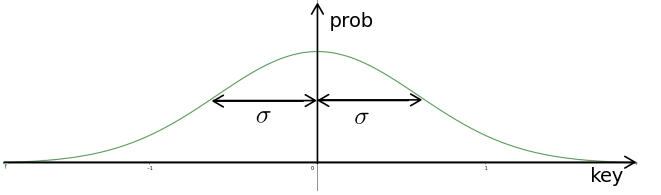
\includegraphics[width=7cm,height=3cm,keepaspectratio]{./Pictures/Graph1.png}\\
                \hspace*{-1cm}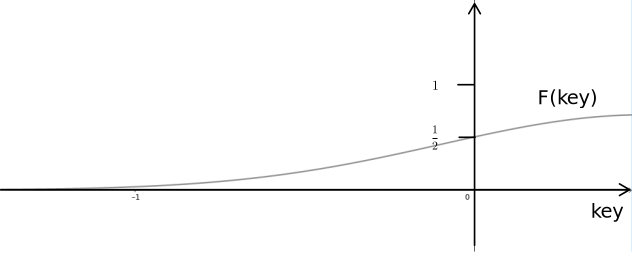
\includegraphics[width=7cm,height=3cm,keepaspectratio]{./Pictures/Graph2.png}\\
            \end{minipage}
        \end{figure}
    \end{itemize}
        \item[b)] keine Formel: empirische Wahrscheinlichkeit $\widehat{=}$ Histogramm \\
        \begin{figure}[htbp]
            \begin{minipage}[t]{10cm}
                \centering
                \vspace{0cm}
                \hspace*{-1cm}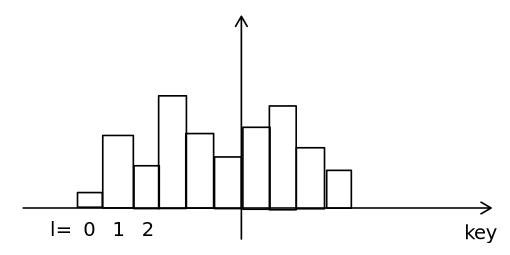
\includegraphics[width=7cm,height=3cm,keepaspectratio]{./Pictures/Balken1.png}\\
            \end{minipage}
            \begin{minipage}[t]{6cm}
            Quantisiere Schlüssel in L Bins\\
            zähle Häufigkeit der Schlüssel für jeden Bin:\\
            \[ h_l \in [0,1]\]
            \end{minipage}
        \end{figure}

        \begin{figure}[htbp]
            \begin{minipage}[t]{10cm}
                \centering
                \vspace{-1cm}
                kumulatives Histogramm $F_e = \sum_{l' = 0}^{l} h_{e'}$ \\
            \end{minipage}
            \begin{minipage}[t]{6cm}
                \hspace*{-1cm}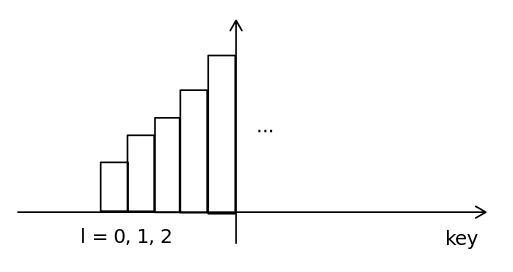
\includegraphics[width=7cm,height=3cm,keepaspectratio]{./Pictures/Balken2.png}\\
            \end{minipage}
        \end{figure}


        $\Rightarrow$ optimale Quantisierung: \hspace*{5mm} l=raw\_quantize(key),
        k = int($F_e * M$)\hspace*{5mm}  F[l] \\

        Hausaufgabe: optimale Quantisierung für Fall a) finden \& bucket\_sort implementieren \\
        Die Quantize-Funktion sollte möglichst billig sein.
\end{enumerate}

